\chapter{Fundamentos Teóricos}
\label{chap:ft}
En este capítulo se repasan los principios básicos sobre los que se establece este trabajo.
\section{Tomografía Computerizada}
\lettrine{U}{na} \acrfull{tc} en esencia, es una máquina de rayos X en la cual se ha sustituido la placa por una serie de detectores\cite{muniz2006introduccion}. El tubo de Rx emite un haz colimado que atraviesa al paciente. De dicho tubo emerge el haz atenuado remanente que es recibido por el detector mientras efectúa un movimiento circular y avanzando lentamente hasta cubrir el área deseada como se puede ver en \ref{fig:tac}.
\begin{figure}%
    \centering
    \subfloat[\centering Orientación del tubo de rayos X respecto al eje corporal.]{{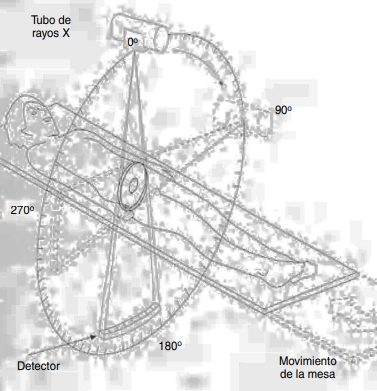
\includegraphics[width=5cm]{imaxes/tac.png} }}%
    \qquad
    \subfloat[\centering Tomografía axial computerizada convencional.]{{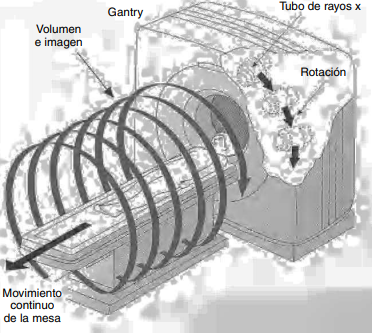
\includegraphics[width=5cm]{imaxes/tacm.png} }}%
    \caption{Representación del funcionamiento de un \acrshort{tc}}%
    \label{fig:tac}%
\end{figure}

\subsection{Teorema de Radon}
El Teorema de Radon, propuesto por el matemático austríaco Johann Radon en 1917, es un resultado fundamental en la teoría de la tomografía computerizada. Este teorema establece que es posible reconstruir una función bidimensional a partir de sus proyecciones a lo largo de diferentes ángulos. En el contexto de la tomografía computerizada, las proyecciones se obtienen mediante la medición de la atenuación de la radiación a medida que atraviesa el objeto en estudio. El Teorema de Radon proporciona la base matemática para la reconstrucción de imágenes en la tomografía computerizada y ha llevado al desarrollo de diversos algoritmos de reconstrucción.

\subsection{Algoritmos de reconstrucción de imágenes}
Los algoritmos de reconstrucción de imágenes son métodos computacionales utilizados para reconstruir imágenes bidimensionales o tridimensionales a partir de proyecciones adquiridas en la tomografía computerizada. Estos algoritmos se basan en el Teorema de Radon y pueden clasificarse en dos categorías principales: métodos analíticos \cite{kontaxakis2002reconstruccion} y métodos iterativos \cite{Willemink2013}.

1. Métodos analíticos: Estos algoritmos, como la retroproyección filtrada (FBP, por sus siglas en inglés), procesan las proyecciones de manera directa para obtener la imagen reconstruida. La FBP es el algoritmo más utilizado en la práctica clínica debido a su rapidez y eficiencia.

2. Métodos iterativos: Estos algoritmos, como el de máxima verosimilitud de la expectativa-maximización (MLEM) y el de mínimos cuadrados conjugados (CGLS), utilizan un enfoque iterativo para mejorar la calidad de la imagen reconstruida. Aunque estos métodos suelen ser más lentos que los analíticos, pueden proporcionar imágenes de mayor calidad y son especialmente útiles en aplicaciones donde la cantidad de datos de proyección es limitada o ruidosa.



\section{Impresión 3D}

La impresión 3D es una tecnología de fabricación aditiva que permite crear objetos tridimensionales a partir de un modelo digital. Esta tecnología ha revolucionado la forma en que se fabrican piezas y productos, ya que permite la creación de objetos complejos con geometrías que serían difíciles o imposibles de lograr con métodos de fabricación tradicionales. La impresión 3D se utiliza en una amplia variedad de aplicaciones, desde la fabricación de piezas de repuesto hasta la creación de prótesis médicas personalizadas.

\subsection{Fabricación aditiva}

La impresión 3D es un ejemplo de fabricación aditiva, que se refiere a manipulación y deposito de un material a escala micrométrica de forma muy precisa para construir un sólido. La fabricación aditiva es una alternativa a los métodos de fabricación tradicionales, como el fresado y el torneado, que implican la eliminación de material de una pieza bruta \cite{zahera2012fabricacion}.

Esta técnica de fabricación presenta una serie de ventajas. La complejidad de la geometría de la figura no encarece la fabricación de la misma (a expensas de la necesidad de material como soporte de la geometría principal) si no que permite generar piezas con geometrías previamente inviables, o con un alto coste.
Otra de las ventajas es la posibilidad de generar prototipos de piezas cuyas versiones finales presentan un alto coste, por un precio muy reducido, y una alta fidelidad acelerando así el proceso iterativo del diseño.

\subsection{Modelado}

El proceso de impresión 3D comienza con el modelado de la pieza o producto que se desea imprimir. Este modelo puede generar utilizando software \acrfull{cad} o mediante la digitalización de un objeto existente utilizando un escáner 3D. 

\subsection{Slicing}
Un modelo 3D es no deja de ser una representación de un archivo de texto plano adaptada para que podamos trabajar con la misma de una forma más sencilla, pero una impresora 3D necesita una serie de instrucciones precisas que seguir para generar una pieza a partir de un modelo. Esta es la función de un programa de Slicing.
En cierto modo podemos considerar este programa como una interfaz entre las personas y las impresoras, ya que permiten realizar ajustes con el fin de obtener el resultado deseado. 
Una vez se ha parametrizado correctamente el volumen que deseamos imprimir, el programa genera una serie de instrucciones precisas que la impresora entiende para elaborar capa a capa el volumen.


\section{Realidad aumentada}

La realidad aumentada es una tecnología que combina elementos virtuales con el mundo real, permitiendo a los usuarios interactuar con objetos y escenarios virtuales en tiempo real. La realidad aumentada se utiliza en una amplia variedad de aplicaciones, desde juegos y entretenimiento hasta la educación y la medicina.

\subsection{Visión Artificial}

Se denomina visión artificial al campo que incluye los métodos necesarios para adquirir, procesar, analizar y comprender las imágenes del mundo real con el fin de producir información procesable por un ordenador. Esta fuertemente vinculado con la realidad aumentada, ya que es imprescindible para poder transmitir la información del medio al ordenador encargado de generar imágenes correspondientes. 
Entre los objetivos de la visión artificial se encuentra la capacidad de reconocer patrones dentro de una imagen o vídeo con el fin de poder extraer las características de los objetos dentro de dicho medio y  procesarlas. 
Otro objetivo es la reconstrucción 3D a partir de imágenes, que pretende generar volúmenes 3D desde las imágenes obtenidas, esto es especialmente importante en la realidad aumentada por que permite una mayor percepción de la profundidad sobre el medio generado por ordenador.